\hone{Allgemeines}
\sectionauthor{Julian Kusternigg}

\htwo{Einführung}

%TODO: Titel vereinheitlichen und \ZELIA verwenden!! č und ć vereinheitlichen!!!
Das "Zentrale, einheitliche Lehrrauminformationsauslesystem", kurz \ZELIA, ist vereinfacht gesagt ein Programm, mit dem man Informationen von Lehrräumen abfragen und verändern kann. Das Ziel von \ZELIA\ ist es, in Schulen verwendet zu werden, um schnell allgemeine Informationen über Räume zu erlangen, ohne sich an Lehrer*innen wenden zu müssen. Da \ZELIA\ im "Schulzentrum Ungargasse" entwickelt wurde, beziehen sich Tests und Beispiele oft auf dieses. Die Anwendung des Programmes ist jedoch ortsunabhängig, da die einzige Voraussetzung zur Verwendung eine eindeutige Raumkennung ist. Somit könnte man \ZELIA\ auch in anderen Schulen ausrollen und verwenden. 

\begin{figure}[H]
    \centering
    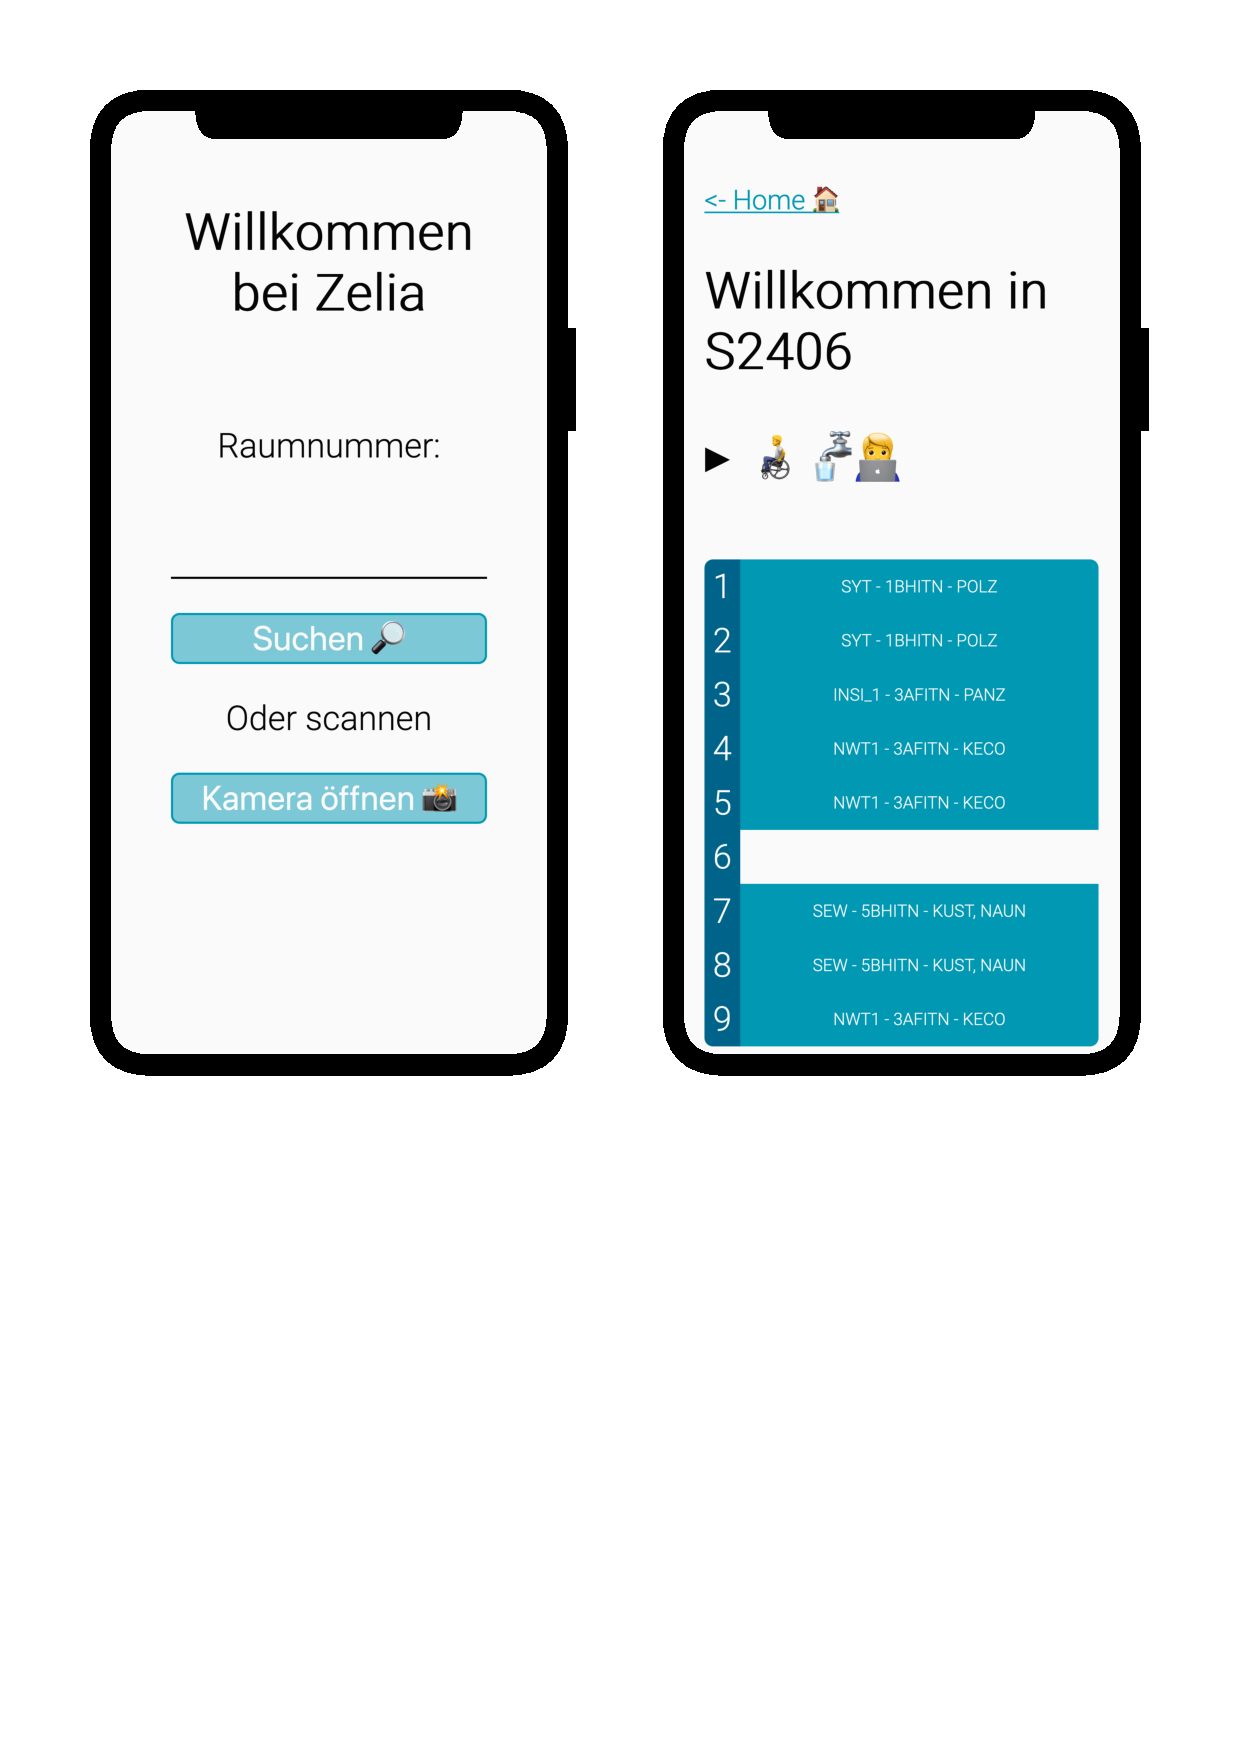
\includegraphics[width=120mm]{media/Intro/frontend_mobile.svg.pdf}
    \caption{Mobilansicht der Web-Applikation}
\end{figure}

Die Benutzeroberfläche von \ZELIA\ läuft als Web-Applikation. Das bedeutet, dass man nur einen Browser braucht, mit dem man die Seite aufrufen und verwenden kann. Das Backend läuft in sogenannten Docker-Containern, welche es ermöglichen, den Server unabhängig von der verwendeten Hardware zu starten (siehe Kapitel Containertechnologie und Docker \ref{sec:ContainerAndDocker}, Seite \pageref{sec:ContainerAndDocker}).

Informationen über einen Raum kann man mit der jeweiligen Raumnummer einfach in der Web-Applikation abfragen. Bei diesen Informationen handelt es sich zum einen um Standarddaten eines Raumes. Zum Anderen werden die Raumstundenpläne von WebUntis abgefragt, damit man immer den aktuellen Stundenplan sehen kann. Die Standarddaten eines Raumes sind zum Beispiel die Anzahl von Plätzen und Computern in einem Raum oder welche Arten von Tafeln sich in diesem befinden.

Neben dem Abfragen von Rauminformationen kann man mit \ZELIA\ auch Anmerkungen zu Räumen erstellen. Dadurch kann man Defekte oder Mängel in Räumen melden. Zusätzlich kann man freie Räume buchen, um diese für Nachhilfe oder andere Zwecke verwenden zu können. Diese Meldungen und Buchungen können von "Administratoren" in der Web-Anwendung angesehen und auch abgearbeitet werden. Bei diesen Administratorbenutzern handelt es sich um Lehrer*innen, welche die Räume verwalten. Dadurch können entweder bestimmte Klassenräume von befugten Lehrern, sprich Administratoren, verwaltet werden oder alle Räume werden von einer Person verwaltet.

Damit man eine Meldung oder Buchung tätigen kann, muss man eine E-Mail-Adresse angeben. Im Fall von \ZELIA\ im Schulzentrum Ungargasse ist dies eine Schul-E-Mail-Adresse. An die angegebene E-Mail-Adresse wird ein Bestätigungslink geschickt und erst wenn dieser aufgerufen wird, ist die Meldung oder Buchung genehmigt. Dadurch wird verhindert, dass man sich einen Account anlegen muss, um solche Anfragen zu stellen. Trotzdem ist nachvollziehbar, welche Schüler*innen Defekte gemeldet haben oder von wem welcher Raum gebucht wurde. Dieses Konzept wird bei \ZELIA\ auch deshalb verwendet, da sich Schüler*innen keinen Account anlegen möchten oder sich mühsam mit einem vorgegebenen Benutzer anmelden wollen. Die Schul-E-Mail-Adressen sind für die Authentifizierung somit viel komfortabler. Es kann passieren, dass Schüler*innen sich einen Spaß erlauben und nicht ihre eigene E-Mail-Adresse angeben. Dadurch würde irgendjemand eine E-Mail bekommen, die nicht gewünscht ist. Dieses Problem gibt es nicht nur bei \ZELIA. Schüler*innen können \zb\ Lehrpersonal so viele E-Mails schicken wie sie wollen. Mit einem Ordner im E-Mail Postfach könnte man alle \ZELIA-E-Mails gruppieren, um einen besseren Überblick im Postfach behalten zu können. Außerdem könnte man die Anzahl der Meldungen und Buchungen, die in einem Zeitintervall gemacht werden dürfen, limitieren, um Spam zu verhindern. Wenn nun eine Buchung akzeptiert oder abgelehnt wird, bekommt man eine E-Mail mit einem Informationstext geschickt, ob man den Raum benutzen darf oder die Anfrage abgelehnt wurde.

ZELIA ist spezifisch für Schulen entwickelt und somit besteht die Zielgruppe vor allem aus Schüler*innen und Lehrer*innen, die täglich in mehreren Lehrräumen unterwegs sind. Für diese Leute ist es oft praktisch zu sehen, in welchem Raum sie später vielleicht sein werden und welche technischen Mittel dort zur Verfügung stehen. Auch für Besucher*innen, wie zum Beispiel an einem "Tag der offenen Tür", könnte \ZELIA\ von Nutzen sein. So könnte man ohne Begleitung durch die Schule gehen und Informationen über Räume und \zb\ Projekte in diesen erfahren.

\begin{minipage}{\textwidth}
    Aufteilen kann man \ZELIA\ in drei Teile: 
    \begin{itemize}
        \item Server
        \item Datenbank
        \item Client
    \end{itemize}
    Jeder dieser Teile ist einzeln geplant und implementiert worden.
\end{minipage}

\begin{figure}[H]
    \centering
    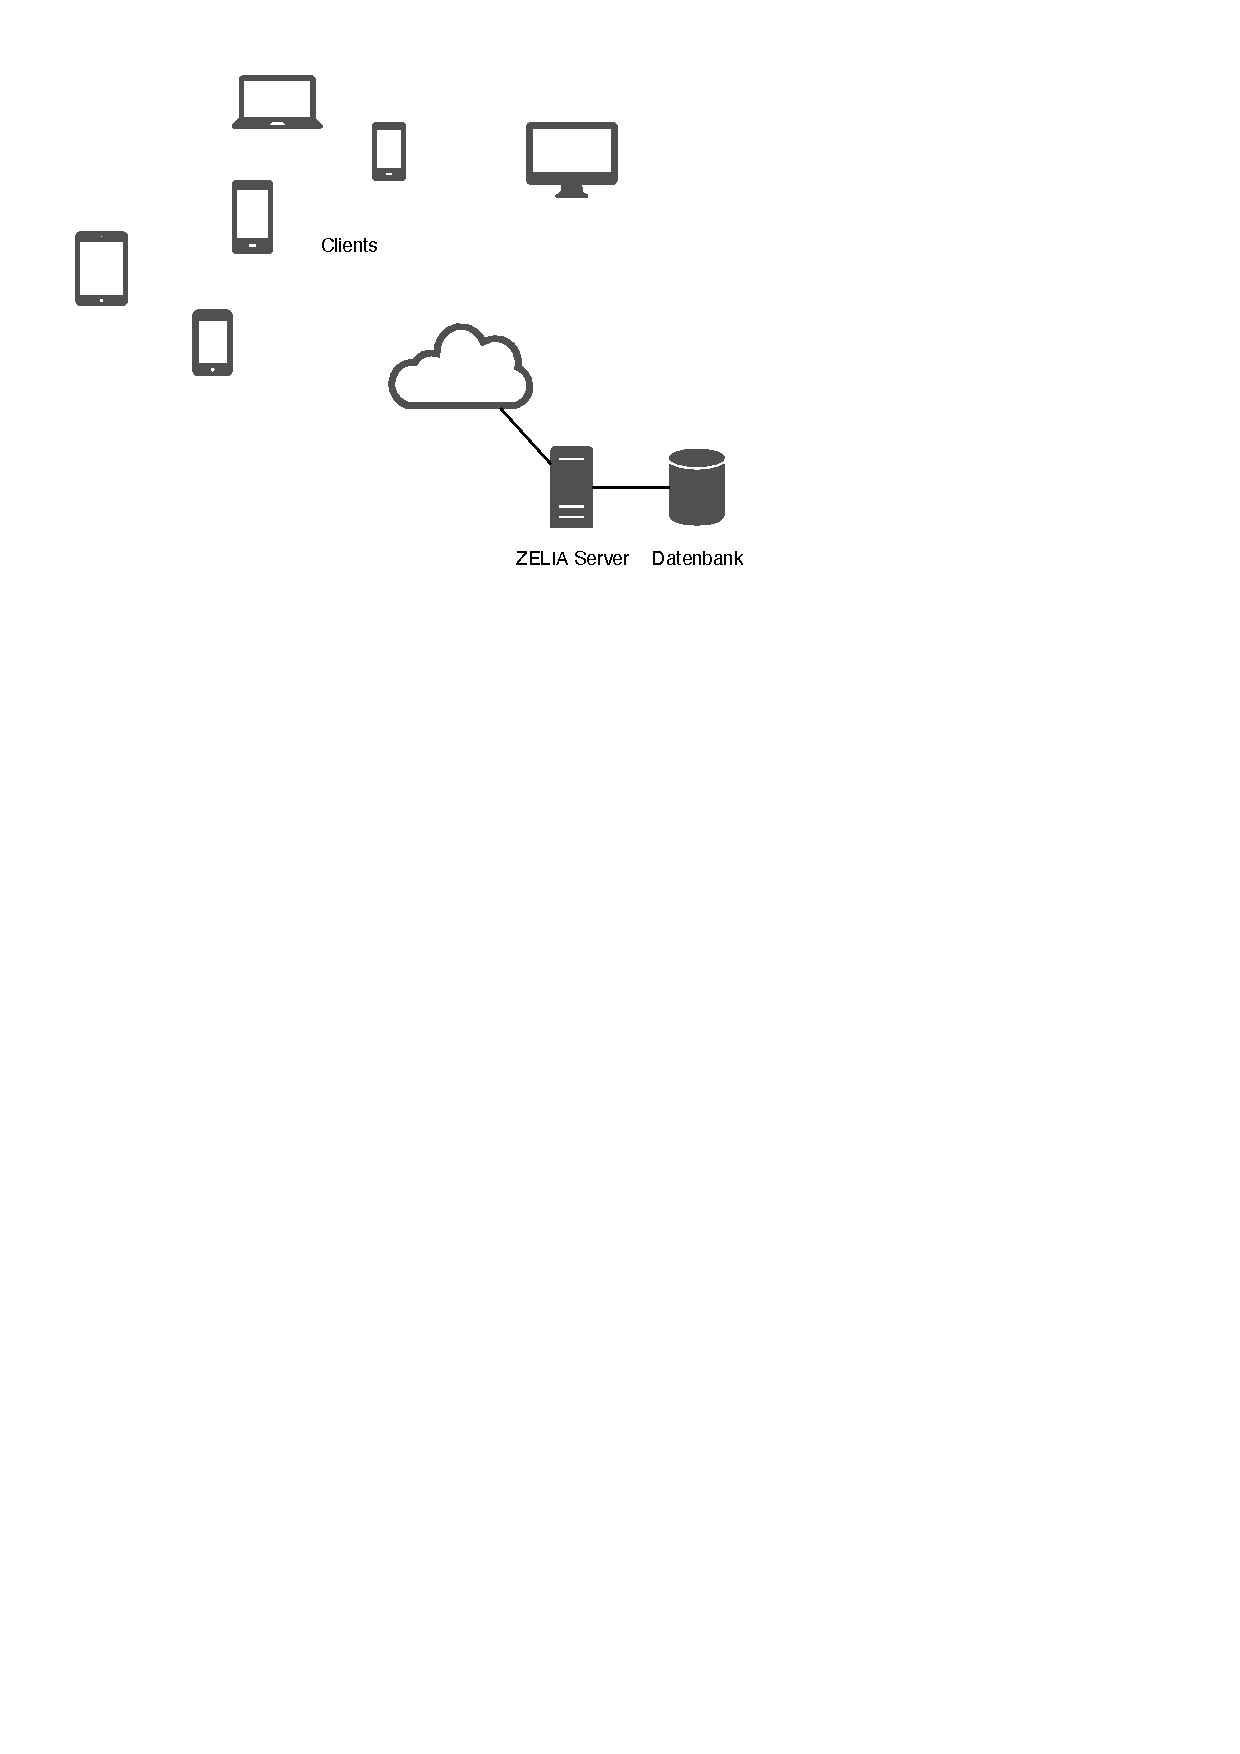
\includegraphics[width=120mm]{./media/Intro/client_server_arch.svg.pdf}
    \caption{Server-Client-Verbindung}
\end{figure}

\htwo{Server}

Der \ZELIA-Server ist der Hauptteil von \ZELIA. Er sammelt und stellt Daten, die benötigt werden, um die Software auf den Endgeräten darstellen zu können, zur Verfügung. Dafür wird der Server nochmal unterteilt.

\begin{itemize}
    \item Der erste und wichtigste Teil ist die Schnittstelle für die Endgeräte, genannt \ZELIA-API ("Application Programming Interface"). Über diese Schnittstelle fragt das Client-Programm Informationen über Räume ab oder sendet Meldungs- und Buchungsanfragen aus.
    \item Der zweite Teil ist die Schnittstelle zwischen Server und Datenbank. Primär werden aus der Datenbank Informationen über Räume abgefragt. Auch andere Daten wie Administratorbenutzer, um Meldungen und Buchungen zu verwalten, stehen in der Datenbank zur Verfügung. 
    \item Der dritte Teil kümmert sich um die Abfragen von WebUntis, um Zugriff auf aktuelle Stundenpläne jeweiliger Räume zu bekommen.
\end{itemize}

Aus der Sicht des Clients ist das Backend ein einzelner Server, wobei dieser eigentlich aus mehreren sogenannten Docker-Containern besteht. Dadurch ist es möglich, die Datenbank und die \ZELIA-API am selben Server in Containern laufen zu lassen. Ein großer Vorteil daran ist, dass man \ZELIA\ als gesamtes System starten und verwalten kann. Gerade in der Entwicklung ist das sehr wichtig, da somit auf jedem beliebigen Computer eine eigene \ZELIA-Instanz gestartet werden kann. Für diese Container macht es keinen Unterschied, ob sie nebeneinander am selben Server laufen oder nicht. Sie sind miteinander über ein virtuelles Netz verbunden (mehr zu Containertechnologie und Docker in Kapitel \ref{sec:ContainerAndDocker}, Seite \pageref{sec:ContainerAndDocker})

\begin{figure}[H]
    \centering
    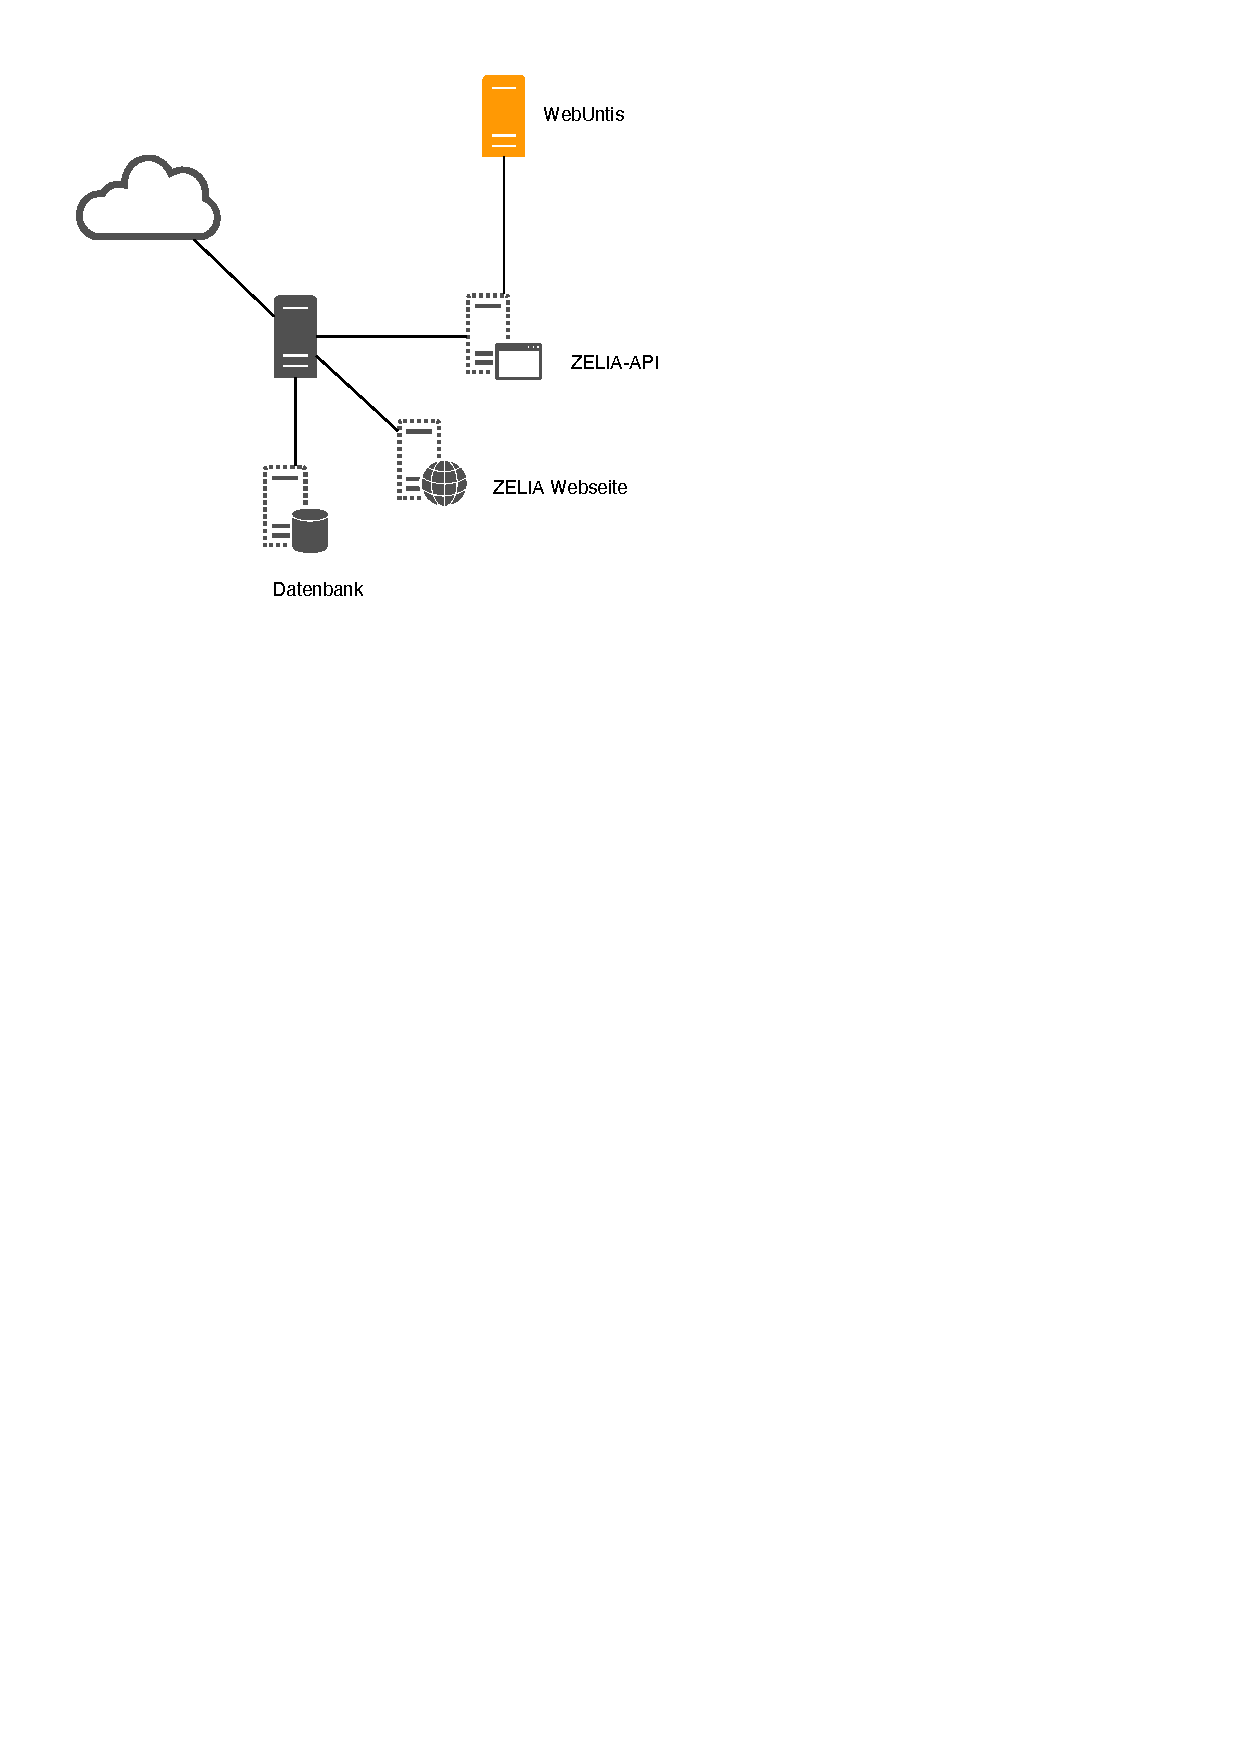
\includegraphics[width=120mm]{./media/Intro/server_arch.svg.pdf}
    \caption{Aufbau des \ZELIA-Servers}
    \label{fig:server_arch}
\end{figure}

Der \ZELIA-API Server ist mittels NodeJS implementiert. NodeJS ist ein Javascript-Framework, welches es ermöglicht einfach mit dem Frontend zu kommunizieren. Außerdem gibt es viele vorgefertigte Pakete, um schnell ein stabiles Backend zu entwerfen. Statt Javascript wird bei \ZELIA\  TypeScript verwendet, welches in Javascript umgewandelt wird. Was genau TypeScript ist und warum es bei \ZELIA\ verwendet wird, ist in Kapitel TypeScript \ref{sec:TypeScript} (Seite \pageref{sec:TypeScript}) erläutert.

\htwo{Datenbank}

Die \ZELIA-Datenbank ist physisch gesehen ein Teil des \ZELIA-Servers (siehe Abbildung \ref{fig:server_arch}). Alle Informationen zu Räumen, wie die Anzahl von Plätzen oder Computern, werden in ihr gespeichert. Dort sind auch Meldungen und Buchungen von Räumen abgelegt, damit später darauf zurückgegriffen werden kann. Diese Meldungen und Buchungen können von Administratorbenutzern abgefragt werden. Diese Administratoren sind in der Datenbank gespeichert. Die Datenbank ist mittels Containertechnologien (siehe Kapitel Containertechnologie und Docker \ref{sec:ContainerAndDocker}, Seite \pageref{sec:ContainerAndDocker}) in einem privaten Netz abgeschottet. Sie kann nur über definierte Schnittstellen vom Server angesprochen und abgefragt werden (siehe Kapitel \ZELIA-API \ref{sec:zeliaapi}, Seite \pageref{sec:zeliaapi}). Für die Datenbankschnittstelle des \ZELIA-Servers wird "Sequelize" verwendet, um Abfragen zu machen (siehe Kapitel Sequelize \ref{sec:sequelize}, Seite \pageref{sec:sequelize}). Verwendet wird die Datenbank "MariaDB" (siehe Kapitel MariaDB \ref{sec:MariaDB}, Seite \pageref{sec:sequelize}).


\htwo{Client}

Damit \ZELIA\ einfach zu verwenden ist, baut der Client auf modernen Web-\-Techno\-logien auf. Somit ist der \ZELIA-Client eine Web-Anwendung,  die von jedem Gerät verwendet werden kann, egal ob Computer, Tablet oder Smartphone. Da \ZELIA\ für die mobile Verwendung konzipiert ist, ist die Web-Applikation so optimiert, dass sie auch auf leistungsschwächeren Geräten und Smartphones gut funktioniert (siehe Kapitel OCR-Modul \ref{sec:ocrmodul}, Seite \pageref{sec:ocrmodul}). Das Frontend wurde mit Fokus auf eine einfache Verwendung auf Smartphones entwickelt, da es durch die Kameras dieser Endgeräte ein wichtiges Feature gibt. Mit der Kamera kann man Raumnummern, zum Beispiel von Türschildern, einscannen. Normalerweise müsste man die Raumnummer selbst eingeben, um die Informationen von einem Raum zu bekommen. 

Nachdem man auf der Startseite eine Raumnummer eingegeben hat, egal ob manuell oder automatisiert durch Einscannen, sieht man die jeweiligen Informationen eines Raumes. Wie schon erwähnt, gibt es auch die Möglichkeit, Räume zu buchen oder Informationen über diese zu melden. Buchungen und Meldungen können im sogenannten "Admin Dashboard" angesehen und nach Relevanz gefiltert werden. Auf diese Administratorübersicht kann auch über die Web-Anwendung zugegriffen werden. Dafür ist ein gültiger Benutzername und Passwort eines Administrators, welcher in der Datenbank gespeichert ist, nötig.

Das Frontend von \ZELIA\ ist von Grund auf mit HTML5 und CSS3 realisiert. Statt Javascript wird auch hier TypeScript verwendet, welches in normales, vom Browser interpretierbares, Javascript umgewandelt wird. 

Das Frontend läuft mit Ausnahme von TesseractJS ohne fremde Bibliotheken (siehe Kapitel Tesseract \ref{sec:tesseract}). TesseractJS wird verwendet, um einen Text aus Bildern auszulesen. Dies wird benötigt, um mit der Kamera eines Endgerätes Raumschilder einscannen zu können. Die Verwendung anderer Bibliotheken wurden aus folgenden Gründen vermieden:
\begin{itemize}
    \item Bibliotheken, wie zum Beispiel Angular, sind für den Anwendungsfall an \ZELIA\ zu groß. Dadurch könnte die Webseite schnell zu komplex und langsam werden.
    \item Um Erfahrungen zu sammeln, wie man eine eigene einfache Bibliothek entwickeln kann, welche nicht nur für die Anwendung an \ZELIA\ konzipiert ist.
\end{itemize}

\begin{minipage}{\textwidth}
    Somit wurden zwei separate Teile entwickelt, auf denen der \ZELIA-Client basiert:
    
    \begin{itemize}
        \item Ein Web-Komponentensystem, um den Inhalt der jeweiligen Seite anzuzeigen (siehe Kapitel \ref{sec:webcomponents}).
        \item Ein Client-Side-Router, um den Inhalt auf mehrere Seiten zu verteilen und zu verwenden (siehe Kapitel \ref{sec:csrouter}).
    \end{itemize}
\end{minipage}
